\chapter{La gestion des points}

\section{Projection d'un point}
Dans la partie \ref{capture de points}, nous verrons que la capture de points n'est pas très précise. En effet, pour deux trajets réalisés sur le même parcours, on peut avoir des points situés à des endroits différents et pris à des intervalles différentes. La figure \ref{Représentation des trajets} représente cet écart lors de la capture des points. Afin de pouvoir comparer deux trajets, nous devons projeter les points (ici le point $A$) du trajet réalisé ($t_2$) sur le trajet de référence ($t_1$). Pour cela nous devons calculer les coordonnées du point $H$ pour déterminer le rapport entre $[BH]$ et $[BC]$ et permettre une estimation du temps établi pour atteindre le point $A$ sur le trajet $t_1$. Nous pourrons ainsi comparer les temps mis pour atteindre les points $A$ sur $t_2$ et $H$ sur $t_1$.

\begin{img}  
	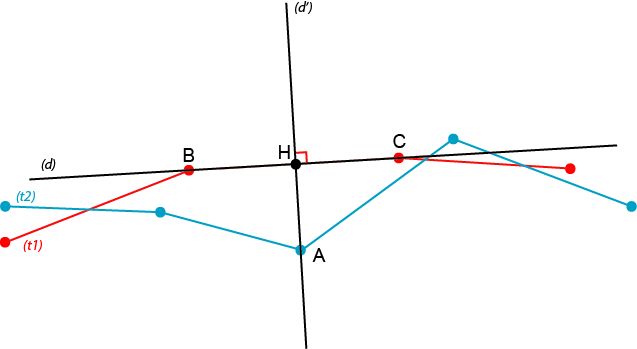
\includegraphics[scale=1]{img/Trajet.png}
	\caption{Représentation des trajets}
	\label{Représentation des trajets}
\end{img}

\subsection{Détermination des coordonnées du projeté}
On pose trois points $ A(x_a,y_a) $, $ B(x_b,y_b) $ et $ C(x_c,y_c) $ et nous cherchons à calculer les coordonnées de $ H(x_h,y_h) $ (Figure \ref{Représentation des trajets}).
Pour ce faire, nous devons commencer par calculer l'équation de la droite $ d $ passant par les points $B$ et $C$.
On pose donc : 
\[
 	d(x) = mx + n
\]
On cherche à déterminer le coefficient directeur de la droite ($m$). Comme $B \in d$ et $C \in d$, on a :
\[
   m =  \frac{x_b-x_c}{y_b-y_c}
\]
Comme le point $B \in (d)$, il résout l'équation :
\[
   y_b = mx_b + n \\
   \Leftrightarrow n = y_b - mx_b
\]
On cherche maintenant à déterminer l'équation de la droite $ d' $ passant par $ A $ tel que $ (d)\bot (d') $. On pose alors, 
\[
 	d'(x) = m'x + n'
\]
Comme $d$ et $d'$ sont orthogonales le produit de leur coefficient directeur est égal à 1, donc:
\[
	mm' = 1 \Leftrightarrow m' = -\frac{1}{m}	
\]
d'où
\[
	d'(x) = -\frac{1}{m}x+n'
\]
et comme $ A \in d' $, on a:
\[
	y_a = -\frac{1}{m}x_a + n' \Leftrightarrow n' = y_a + \frac{1}{m}x_a
\]
Comme $ H \in d$ et $H \in d'$, il résout le système suivant :
\begin{align}
    &\begin{cases}
   		 & y_h = -\dfrac{1}{m}x_h + n'\\
   		 & y_h = mx_h + n
    \end{cases} 
    \Leftrightarrow
    \begin{cases}
   		& x_h = -my_h + mn'\\
    	& y_h = mx_h + n
    \end{cases} 
    \Leftrightarrow
    \begin{cases}
   		& x_h = -my_h + mn'\\
    	& y_h = -y_hm^2 + m^2n' + n
    \end{cases} \\
    \Leftrightarrow
    \label{systeme}
    &\begin{cases}
   		& x_h = \dfrac{(m^2+n'+n)m}{m^2+1} + n'm \\
    	& y_h = \dfrac{(m^2+n'+n)m}{m^2+1}
    \end{cases}
\end{align}
En remplaçant les valeurs dans l'équation \eqref{systeme}, on obtient :

\begin{align}
	\begin{cases}
		 x_h = \dfrac{\left( \dfrac{x_b - x_c}{y_b - y_c}\right)^2 + y_b - \left( \dfrac{x_b - x_c}{y_b - y_c}\right) x_b + y_a + \left( \dfrac{y_b - y_c}{x_b - x_c}\right) x_a}{\left( \dfrac{x_b - x_c}{y_b - y_c}\right)^2 + 1} + \left( y_a + \left( \dfrac{y_b - y_c}{x_b - x_c}\right) x_a\right) \left( \dfrac{x_b - x_c}{y_b - y_c}\right)  \\
    	 y_h = \dfrac{\left( \dfrac{x_b - x_c}{y_b - y_c}\right)^2 + y_b - \left( \dfrac{x_b - x_c}{y_b - y_c}\right) x_b + y_a + \left( \dfrac{y_b - y_c}{x_b - x_c}\right) x_a}{\left( \dfrac{x_b - x_c}{y_b - y_c}\right)^2 + 1}
	\end{cases}
\end{align}

\subsection{L'interpolation temporelle}
Après avoir récupérer les coordonnées du projeté, nous pouvons calculer le rapport ($\theta$) entre la distance $BH$ et $HC$ et l'appliquer au temps établi pour parcourir la distance $BC$ ($\Delta_{BC}$) afin d'estimer l'interpolation du temps au point $H$. Donc
\[
	t_H = \frac{distance(B,H)}{distance(B,C)}| t_B - t_C | 
\]
Nous pouvons alors comparer le temps mis pour atteindre $A$ et le temps mis pour atteindre $H$.
\begin{align}
\mbox{Si } t_H - t_A &<0 \mbox{ On est en avance.} \\
			&>0 \mbox{ On est en retard.} \\
			&=0 \mbox{ On est pareil.}
\end{align}

\section{Recherche du segment pour effectuer la projection}
\subsection{Vérification du projeté dans le segment}
Dès lors que les coordonnées du point $H$ sont trouvées, nous devons vérifier que $H$ appartient au segment $[BC]$. En effet, si la projection n'est pas située sur le bon segment, les résultats vont devenir incohérents. On admettra donc l'existence d'une méthode \verb!estSurSegment! permettant de vérifier que $H$ est bien compris sur le segment $[BC]$.

\subsection{L'algorithme de détermination des projetés}
Voyons maintenant l'algorithme permettant, à partir d'une liste de points géolocalisés, d'établir une liste de ses projetés sur un des points référencés.
\begin{algorithmic}
\Function {CalculProjection}{Points[] $t_{act}$, Points[] $t_{ref}$}
\Initialize{$i_{ref} \gets 0$\\$i_{act}\gets 0$\\$projections[t_{act}.size()]$\\$projete\gets null$}
\While{($i_{ref} < t_{ref}.size()-1$ and $i_{act} < t_{act}.size()$ )}
	\State $projete \gets calulProjection(t_{act}[i_{act}],t_{ref}[i_{ref}],t_{ref}[i_{ref}+1])$
    \If{($estSurSegment(projete, t_{ref}[i_{ref}], t_{ref}[i_{ref}+1])$)}
    	\State $projection[i_{act}]\gets projete$
    	\State $i_{act}\gets i_{act}+1$
   	\Else
   		\State $i_{ref}\gets i_{ref}+1$
    \EndIf

\EndWhile
\EndFunction
\end{algorithmic}

\section{Les problèmes rencontrés}
Analytiquement parlant, tout semble fonctionner correctement, mais lors de l'implémentation nous nous sommes rendu compte de plusieurs problèmes. 

\subsubsection{Division par zéro}
Lors du calcul des coordonnées du projeté, les points du segment ne doivent pas avoir la même latitude ou longitude. Si tel est le cas, ils seront alignés et leur différence d'abscisse ou d'ordonnée sera nulle. On diviserait alors par zéro lorsque l'on calcule les coefficients directeurs des droites.

\subsubsection{Projeté impossible}
Dans l'algorithme présenté précédemment, nous nous sommes rendu compte que si un des points ne pouvait pas être projeté, la suite de l'algorithme était complètement inutile. Ce cas est plus problématique que le précédent car nous n’avons pas trouvé de moyen simple pour le résoudre.

\subsubsection{Mauvais projeté}
Nous nous sommes également rendu compte que dans certain cas, un point pouvait être projeté sur plusieurs segment. Dans ce cas la, le point peut être projeté sur un mauvais segment donnant ainsi des résultats aberrants en termes de temps. La comparaison est alors totalement inutile.